%#% extstart input preamble.tex
%
% memman.tex  Memoir class user manual (Part II only)  last updated 2009/09/07
%             Author: Peter Wilson
%             Copyright 2001, 2002, 2003, 2004, 2008, 2009 Peter R. wilson
%
%   This work has the LPPL maintenance status "maintained".
%   Maintainer: Lars Madsen (daleif at math dot au dot dk)
%
%\listfiles
\documentclass[10pt,letterpaper,extrafontsizes]{memoir}
\listfiles
\usepackage{comment}


% For (non-printing) notes  \PWnote{date}{text}
\newcommand{\PWnote}[2]{} 
\PWnote{2009/04/29}{Added fonttable to the used packages}
\PWnote{2009/08/19}{Made Part I a separate doc (memdesign.tex).}

% same
\newcommand{\LMnote}[2]{} 


\usepackage{memsty}
%%%%%%%%%%%%%%%%%%%%%%%%%%%%
\usepackage{titlepages}  % code of the example titlepages
\usepackage{memlays}     % extra layout diagrams
\usepackage{dpfloat}     % floats on facing pages
\usepackage{fonttable}[2009/04/01]   % font tables
%%%%\usepackage{xr-hyper} \externaldocument{memdesign} Doesn't work, 
%%%%                      Idea won't work in general for memman/memdesign
%%%%                      as at display time, who knows where everything
%%%%                      will be located on the individual's computer.
%%%%%%%%%%%%%%%%%%%%%%%%%%%%

%%%% Change section heading styles
%%%\memmansecheads

%%%% Use the built-in division styling
\headstyles{memman}

%%% ToC down to subsections
\settocdepth{subsection}
%%% Numbering down to subsections as well
\setsecnumdepth{subsection}

%%%% extra index for first lines
\makeindex[lines]


% this 'if' is used to determine whether we are compiling the memoir
% master in the subversion repository, or the public memman.tex
\newif\ifMASTER
\MASTERfalse
%\MASTERtrue

\ifMASTER

% add patch to fink, such that \AtEndFile still work
\makeatletter
\AtEndFile{fink.sty}{
  \typeout{patching fink} 
  \renewcommand{\InputIfFileExists}[2]{%
    \IfFileExists{##1}%
    {##2\@addtofilelist{##1}%
      \m@matbeginf{##1}%
      \fink@prepare{##1}%
      %\@@input \@filef@und
      \expandafter\fink@input%
      \expandafter\fink@restore\expandafter{\finkpath}%
     \m@matendf{##1}%
     \killm@matf{##1}}%
 }
}
\makeatother
% private package, not in circulation
% enables us to gather svn information on a single file basis
%\usepackage[filehooks]{svn-multi-private}
% use the current version
\usepackage[filehooks]{svn-multi}


% \svnidlong
% {}
% {$LastChangedDate: 2015-03-05 18:49:59 +0100 (Thu, 05 Mar 2015) $}
% {$LastChangedRevision: 516 $}
% {$LastChangedBy: daleif $}



\makeatletter
\newcommand\addRevisionData{%
  \begin{picture}(0,0)%
    \put(0,-20){%
      \tiny%
      \expandafter\@ifmtarg\expandafter{\svnfiledate}{}{%
        \textit{\textcolor{darkgray}{Chapter last updated \svnfileyear/\svnfilemonth/\svnfileday
         \enspace (revision \svnfilerev)}}
     }%
    }%
  \end{picture}%
}
\makeatother

% we add this to the first page of each chapter

\makepagestyle{chapter}
\makeoddfoot{chapter}{\addRevisionData}{\thepage}{}
\makeevenfoot{chapter}{\addRevisionData}{\thepage}{}

\else
% disable svn info collecting
\newcommand\svnidlong[4]{}
\fi

% Default fixed font does not support bold face
\DeclareFixedFont{\ttb}{T1}{txtt}{bx}{n}{12} % for bold
\DeclareFixedFont{\ttm}{T1}{txtt}{m}{n}{12}  % for normal

% Custom colors
\usepackage{color}
\definecolor{deepblue}{rgb}{0,0,0.5}
\definecolor{deepred}{rgb}{0.6,0,0}
\definecolor{deepgreen}{rgb}{0,0.5,0}

\usepackage{listings}
\usepackage[numbers]{natbib}
\usepackage{hyperref}
% Python style for highlighting
\newcommand\pythonstyle{\lstset{
language=Python,
basicstyle=\ttm,
otherkeywords={self},             % Add keywords here
keywordstyle=\ttb\color{deepblue},
emph={MyClass,__init__},          % Custom highlighting
emphstyle=\ttb\color{deepred},    % Custom highlighting style
stringstyle=\color{deepgreen},
frame=tb,                         % Any extra options here
showstringspaces=false            % 
}}

\newcommand\pythonstyleexample{\lstset{
language=Python,
title={Example 1},
basicstyle=\ttm,
otherkeywords={self},             % Add keywords here
keywordstyle=\ttb\color{deepblue},
emph={MyClass,__init__},          % Custom highlighting
emphstyle=\ttb\color{deepred},    % Custom highlighting style
stringstyle=\color{deepgreen},
frame=tb,                         % Any extra options here
showstringspaces=false            % 
}}


% Python environment
\lstnewenvironment{python}[1][]
{
\pythonstyle
\lstset{#1}
}
{}

\lstnewenvironment{pythonexample}[1][]
{
\pythonstyleexample
\lstset{#1}
}
{}

% Python for external files
\newcommand\pythonexternal[2][]{{
\pythonstyle
\lstinputlisting[#1]{#2}}}

% Python for inline
\newcommand\pythoninline[1]{{\pythonstyle\lstinline!#1!}}

\newcommand\pythonclass[1]{\textbf{\color{deepred}#1}}

%% end preamble
%%%%%%%%%%%%%%%%%%%%%%%%%%%%%%%%%%%%%%%%%%%%%%%%%%%%%%%
%#% extend

\usepackage[draft]{fixme}
\fxsetup{
  layout=marginnote
}
 

\begin{document}




%#% extstart input intro.tex





%\tightlists
\firmlists
\midsloppy
\raggedbottom
\chapterstyle{demo3}

%%%%%%%%%%%%%%%%%%%%%%%%%%%%%%%%%%%%%%%%%%%%%%%%%%%%%%%


\ProvidesFile{memnoidxnum}[2009/04/30  some index entries for memman]
\newcommand*{\idxat}{\index{@?\texttt{@}|noidxnum}} \idxat
%%\index{@?\texttt{@}|noidxnum}
\index{argument|noidxnum}
%%\index{array|noidxnum}
\index{cardinal|noidxnum}
\index{centering|noidxnum}
%%\index{chapterstyle|noidxnum}
%%\index{counter|noidxnum}
\index{default|noidxnum}
\index{division|noidxnum}
\index{division!sectional|seealso{subhead}}
\index{double column|noidxnum}
\index{endnote!mark|seealso{reference mark}}
\index{environment|noidxnum}
\index{error message|noidxnum}
\index{figures|noidxnum}
%%\index{file|noidxnum}
\index{font characteristic|noidxnum}
\index{footnote!mark|seealso{reference mark}}
\index{footnotes|noidxnum}
\index{frame|noidxnum}
\index{framed|noidxnum}
\index{full stop|seealso{period}}
\index{hanging|noidxnum}
\index{headstyles|noidxnum}
%%\index{horizontal|noidxnum}
\index{Hurenkinder|see{widow}}
\index{interlinear space|see{leading}}
\index{keyword|noidxnum}
%%\index{label|noidxnum}
\index{LaTeX?\ltx|noidxnum}
%%\index{length|noidxnum}
\index{line|noidxnum}
\index{line too long|see{overfull lines}}
\index{lining|noidxnum}
%%\index{list|noidxnum}
\index{lowercase|noidxnum}
\index{MakeIndex?\Pmakeindex|noidxnum}
\index{margin!spine|seealso{inner}}
\index{margin!inner|seealso{spine}}
\index{margin!foredge?\foredge|seealso{outer}}
\index{margin!outer|seealso{\foredge}}
\index{margin!upper|seealso{top}}
\index{margin!top|seealso{upper}}
\index{math|noidxnum}
%%\index{memoir class|noidxnum}
\index{minipage|noidxnum}
\index{name|noidxnum}
\index{named|noidxnum}
\index{new|noidxnum}
%%\index{number|noidxnum}
\index{numeric|noidxnum}
\index{old-style|noidxnum}
\index{option|noidxnum}
\index{ordinal|noidxnum}
\index{outline|noidxnum}
\index{package|noidxnum}
\index{page break|noidxnum}
%%\index{pagestyle|noidxnum}
\index{paragraph break|noidxnum}
\index{period|seealso{full stop}}
\index{poem|noidxnum}
\index{program|noidxnum}
\index{ranging|noidxnum}
\index{reference|noidxnum}
\index{reference mark|seealso{endnote mark, footnote mark}}
\index{representation|noidxnum}
\index{rule|noidxnum}
\index{ruled|noidxnum}
%%\index{section|noidxnum}
\index{Schusterjungen|see{orphan}}
\index{section|seealso{subhead}}
\index{sectional division|seealso{subhead}}
\index{single column|noidxnum}
\index{size|noidxnum}
\index{space|noidxnum}
\index{space!double|see(double spacing)}
\index{space!between lines|see{leading}}
\index{stanza|noidxnum}
%%\index{subfloat|noidxnum}
\index{TeX?\tx|noidxnum}
\index{text|noidxnum}
\index{titling|noidxnum}
\index{trim|noidxnum}
%%\index{type size|noidxnum}
\index{vertical|noidxnum}
\index{warning|noidxnum}
\index{write|noidxnum}
%%\index{XeTeX?\xetx|noidxnum}

%%%%%%%% Deleted the font indexing (now done as typefaces) 2009/04/30

\begin{comment}
\index{table of contents|see{ToC}}
\index{list!of figures|see{LoF}}
\index{figure!list of|see{LoF}}
\index{list!of tables|see{LoT}}
\index{table!list of|see{LoT}}
\index{marginal note|see{marginalia}}
\index{footnote!in title|see{thanks}}
\index{illustration|seealso{float, figure}}
\index{figure|seealso{float}}
\index{table|seealso{float}}
\index{chapter!style|see{chapterstyle}}
\index{chapter!heading|see{heading}}
\index{page!style|see{pagestyle}}
\index{part!heading|see{heading}}
\end{comment}

\begin{comment}

%%%% deleted the \nocites
%
\index{anonymous division|see{division}}
\index{array|seealso{tabular}}
%
\index{Berne Convention|see{copyright}}
\index{blank page|see{page}}
\index{Buenes Aires Convention|see{copyright}}
\index{box!rule|seealso{rule}}
%
\index{chapter|seealso{division}}
\index{chapter!style|see{chapterstyle}}
\index{command|seealso{declaration, macro}}
\index{comptexttex?\texttt{comp.text.tex} newsgroup|see{\ctt}}
\index{Comprehensive TeX Archive Network?\cTeXan|see{\ctan}}
\index{contents list|see{ToC}}
\index{counter representation!Alph tt?\texttt{Alph}|see{\texttt{Alph}}}
\index{counter representation!alph tt?\texttt{alph}|see{\texttt{alph}}}
\index{counter representation!arabic tt?\texttt{arabic}|see{\texttt{arabic}}}
\index{counter representation!Roman tt?\texttt{Roman}|see{\texttt{Roman}}}
\index{counter representation!roman tt?\texttt{roman}|see{\texttt{roman}}}
\index{counter representation!fnsymbol tt?\texttt{fnsymbol}|see{\texttt{fnsymbol}}}
\index{cross reference|seealso{reference}}
%
\index{descriptive list|see{list}}
\index{display math|see{math}}
\index{display mode|see{display}}
\index{division|seealso{heading}}
%
\index{electronic book|see{ebook}}
\index{enumerated list|see{list}}
%
\index{figure!list of|see{LoF}}
\index{figure|seealso{float}}
\index{float!numbered captioning|see{caption}}
\index{float!unnumbered captioning|see{legend}}
\index{font characteristic!weight|see{series}}
%
\index{file|seealso{stream}}
\index{footnote!in title|see{thanks}}
\index{fragile command|seealso{protect}}
\index{free tabular|seealso{tabular}}
%
\index{header|seealso{running header}}
\index{heading|seealso{division}}
%
\index{illustration|seealso{float, figure}}
\index{inline math|see{math}}
\index{International Standard Book Number|see{ISBN}}
\index{itemized list|see{list}}
%
\index{label|seealso{reference}}
\index{left-to-right|see{LR}}
\index{list!new list of|see{list of, new}}
\index{list!of contents|see{ToC}}
\index{list!of figures|see{LoF}}
\index{list!of tables|see{LoT}}
\index{list of!contents|see{ToC}}
\index{list of!figures|see{LoF}}
\index{list of!tables|see{LoT}}
\index{LoF|seealso{ToC}}
\index{LoT|seealso{ToC}}
\index{log-like function|see{function}}
%
\index{macro|seealso{command}}
\index{margin note|seealso{marginalia}}
\index{marginalia|seealso{marginal note, side note, sidebar}}
%
\index{named division|see{division}}
%
\index{page!of floats|see{float, page}}
\index{page!start new|see{start new page}}
\index{page!style|see{pagestyle}}
\index{paragraph|seealso{division}}
\index{part|seealso{division}}
\index{picture object!Bezier curve|see{Bezier curve}}
\index{picture object!circle|see{circle}}
\index{picture object!line|see{line}}
\index{picture object!oval|see{box, rounded}}
\index{picture object!vector|see{vector}}
\index{poem|see{verse}}
\index{poetry|see{verse}}
\index{print run|see{impression}}
\index{protect|seealso{fragile command}}
%
\index{recto|seealso{odd page}}
\index{reference|seealso{label}}
\index{river|see{white space}}
\index{rivulet|see{white space}}
\index{running footer|see{footer}}
\index{running header|seealso{header}}
%
\index{section|seealso{division}}
\index{side note|seealso{marginalia}}
\index{sidebar|seealso{marginalia}}
\index{stanza|seealso{verse}}
\index{stanza!line number|see{line number}}
\index{subparagraph|seealso{division}}
\index{subsection|seealso{division}}
\index{subsubsection|seealso{division}}
%
\index{table of contents|see{ToC}}
\index{table!list of|see{LoT}}
\index{table|seealso{float}}
\index{tabular|seealso{array}}
\index{tabular!free|see{free tabular}}
\index{tabulation|see{tabular}}\
\index{TeX Users Group?\TeXUG|see{\tug}}
\index{textblock|see{typeblock}}
%
\index{Universal Copyright Convention|see{copyright}}
%
\index{verbatim!line number|see{line number}}
\index{verse|seealso{stanza}}
\index{verse!title|see{poem title}}
\index{verse!line number|see{line number}}
\index{verso|seealso{even page}}
\index{visual markup|see{visual design}}
%
\index{x coordinate|see{coordinate}}
%
\index{y coordinate|see{coordinate}}
%
%


\end{comment}

\endinput



\frontmatter
\pagestyle{empty}


% title page
\vspace*{\fill}
\begin{center}
\HUGE\textsf{firedrake - mlmc}\par
\end{center}
\bigskip
\begin{center}
\Huge\textsf{User Guide}\par
\end{center}
\bigskip
\begin{center}
\LARGE\textsf{A. Gregory}\par
\bigskip
\normalsize\textsf{\textit{Imperial College London}}\par
\medskip
\end{center}
\vspace*{\fill}
\def\THP{T\kern-0.2em H\kern-0.4em P}%   OK for CMR
\def\THP{T\kern-0.15em H\kern-0.3em P}%   OK for Palatino

\clearpage



\endgroup

\cleardoublepage

% ToC, etc
%%%\pagenumbering{roman}
\pagestyle{headings}
%%%%\pagestyle{Ruled}

\clearpage
%\setupmaintoc
\tableofcontents
\setlength{\unitlength}{1pt}

%#% extend


%#% extstart include preface.tex
%\chapter{Foreword}

\svnidlong
{$Ignore: $}
{$LastChangedDate: 2014-11-05 16:28:11 +0100 (Wed, 05 Nov 2014) $}
{$LastChangedRevision: 501 $}
{$LastChangedBy: daleif $}

\chapter{Preface}


    This is the documentation manual for the \textbf{firedrake-mlmc} package that comprises of a toolbox of Python algorithms that fit under the multilevel Monte Carlo uncertainty quantification framework for random PDEs using \textbf{firedrake}, an automated finite element solver.\\
    
    The repository can be downloaded from: \\
    \url{https://github.com/firedrakeproject/firedrake-mlmc}
    
{\raggedleft{\scshape Alastair Gregory} \\ Imperial College London \\ 2016\par}


\svnidlong
{$Ignore: $}
{$LastChangedDate: 2015-04-22 17:17:51 +0200 (Wed, 22 Apr 2015) $}
{$LastChangedRevision: 527 $}
{$LastChangedBy: daleif $}

\chapter{Forming Mesh and Function Space Hierarchies}

The first step to using this package is understanding how to use hierarchies of meshes and function spaces alongside \textbf{firedrake}. Suppose we build a \pythonclass{Mesh} on a unit square, and want to use this as the coarsest mesh in a refined hierarchy of $L = 4$ other meshes (so a hierarchy of length $L + 1$). We can do this via the example below, by using a \pythonclass{GeneralisedMeshHierarchy}. Note the \pythonclass{GeneralisedMeshHierarchy} differs from the traditional \textbf{firedrake} multigrid \pythonclass{MeshHierarchy} by allowing the additional option of refining with a factor $M \geq 2$ where this is required to be a factor of $2$. Each \pythonclass{GeneralisedMeshHierarchy} has an attribute \pythonclass{GeneralisedMeshHierarchy.\_hierarchy} corresponding to the M-refined hierarchy of meshes, and \pythonclass{GeneralisedMeshHierarchy.\_full\_hierarchy} corresponding to the full hierarchy of intermediate meshes (with $M = 2$). \\
One can then build \pythonclass{GeneralisedFunctionSpaceHierarchy}s via the following commands:\\

\begin{python}
import firedrake_mlmc as *

# mesh on coarsest level
coarsest_mesh = UnitIntervalMesh(5)

# L and refinement factor
L = 4; M = 2

# define mesh and function space hierarchies 
m = GeneralisedMeshHierarchy(coarsest_mesh, L, M)
fs = GeneralisedFunctionSpaceHierarchy(m, 'DG', 1)
\end{python}

Furthermore these generalised hierarchies are also invariant to the prolong and injection methods that exist in multigrid \textbf{firedrake} currently. For example, given \pythoninline{F = Function(fs[0]).assign(2)} and \pythoninline{G = Function(fs[2])}, one can prolong F to G via \pythoninline{prolong(F, G)}. \\
Just as with their \pythonclass{Mesh} counterparts, a \pythonclass{GeneralisedFunctionSpaceHierarchy} has attributes, \pythonclass{GeneralisedFunctionSpaceHierarchy.\_hierarchy} corresponding to the M-refined hierarchy of functionspaces, and \pythonclass{GeneralisedFunctionSpaceHierarchy.\_full\_hierarchy} corresponding to the full hierarchy of intermediate function spaces (with $M = 2$).

\chapter{Creating States of Coarse and Fine Solutions}

An important aspect of multilevel Monte Carlo is being able to have coupled realisations of random variables (in our case, random discretized fields) from 2 consecutive levels, for example \pythoninline{coarse_lvl} and \pythoninline{fine_lvl}. These are typically coupled due to positive correlation one is required to have between the two of them, such as is usually imparted by using the same random input (e.g. initial condition). To this end, it is important that this package keeps each pair of coupled realisations together. It does this via \pythoninline{State(coarse, fine)}. An example of how to create a \pythonclass{State} is below. 

\begin{python}
# define the coarse and fine levels
coarse_lvl = 0; fine_lvl = 1

# define the coarse and fine functions
coarse = Function(fs[coarse_lvl])
fine = Function(fs[fine_lvl])
\end{python}

At this point, one should use \pythoninline{coarse} and \pythoninline{fine} as the fields to solve the coarse and finer discretization of the random system on. As a demostration of this on an extremely simple random system, we interpolate \pythoninline{sin((x + p) * 2 * pi)} on to \pythoninline{coarse} and \pythoninline{fine} where $p \sim N(0, .1)$. As each couple of realisations have to be positively correlated in the multilevel Monte Carlo framework, one should use the same draw of $p$.\\

\begin{pythonexample}
import numpy as np

def example_system(coarse, fine,
                   coarse_lvl, fine_lvl,
                   m):
    # randomly draw shift
    p = np.random.normal(0, .1, 1)[0]

    # interpolate
    x = SpatialCoordinate(m[coarse_lvl])
    coarse.interpolate(sin((x[0] + p) * 2 * pi))
    x = SpatialCoordinate(m[fine_lvl])
    fine.interpolate(sin((x[0] + p) * 2 * pi))
    
    return coarse, fine
\end{pythonexample}

Now that we have two realisations of our (all be it in this case incredibly simple) 'system', we can combine them in a \pythonclass{State}.\\

\begin{python}
coarse, fine = example_system(coarse, fine,
                              coarse_lvl, fine_lvl,
                              m) 

# build state
S= State(coarse, fine)

# check the levels of the state contents
print S.levels
\end{python}

This object requires \pythoninline{coarse_lvl} and \pythoninline{fine_lvl} to be consecutive levels in the \pythonclass{GeneralisedMeshHierarchy} / \pythonclass{GeneralisedFunctionSpaceHierarchy}. Here, the coarse and fine inputs can be a \pythonclass{Function} or one can use input scalar quantities of interest from functions which have been computed on different levels of the \pythonclass{GeneralisedFunctionSpaceHierarchy} using \pythonclass{Constant}s. \\

\begin{python}
# define the scalar quantities of interest
coarse = Constant(0, domain=m[coarse_lvl])
fine = Constant(0, domain=m[fine_lvl])

# build state
S= State(coarse, fine)
\end{python}

These \pythonclass{Constant}s contain their level information from the specified domain (\pythonclass{GeneralisedMeshHierarchy}) whereas \pythonclass{Function}s in a \pythonclass{State} exist on a \pythonclass{GeneralisedFunctionSpaceHierarchy}.


\chapter{Building an Ensemble Hierarchy}

Now that we can generate a \pythonclass{State} for every realisation in an ensemble corresponding to two consecutive levels in a hierarchy of discretizations, a hierarchy of ensembles need to be able to store these \pythonclass{State}s. Another object, a \pythonclass{EnsembleHierarchy}, is used to do exactly this. It stores the \pythonclass{State}s from each realisation on different levels so that statistics and the outputs of multilevel Monte Carlo can be computed. One can store a state in the \pythonclass{EnsembleHierarchy} using the following commands:\\

\begin{python}
# initialize a hierarchy
hierarchy = EnsembleHierarchy(fs, state_type=Function)

# append state to hierarchy
hierarchy.AppendToEnsemble(S)
\end{python}

Given this logic, one can store $N$ random realisations of a system on one level of the hierarchy via a simple loop. Continuing the earlier example, \\

\begin{pythonexample}
# initialize a hierarchy
hierarchy = EnsembleHierarchy(fs, state_type=Function)

# define coarse and fine level
coarse_lvl = 0; fine_lvl = 1

# define the coarse and fine functions
coarse = Function(fs[coarse_lvl])
fine = Function(fs[fine_lvl])

# store N random realisations of system in ensemble
# hierarchy
for i in range(N):
    coarse, fine = example_system(coarse, fine,
                                  coarse_lvl, fine_lvl,
                                  m)
    S = State(coarse, fine)
    hierarchy.AppendToEnsemble(S)

\end{pythonexample}

Once initialized, the \pythonclass{EnsembleHierarchy} object itself can be indexed to access the stored \pythonclass{State}s. The $n$'th state that is appended to the $l$'th ($l \in [0, L]$) level of the hierarchy will be indexed by \pythoninline{hierarchy[l][n]}. \\

\begin{python}
# display the finer input of the n'th state on
# the coarsest level in the hierarchy
print hierarchy[0][n][1]
\end{python}

This object also carries a lot of useful information about the contents on itself, from the refinement factor of \pythonclass{Mesh}s (\pythoninline{hierarchy.M}) used in the hierarchy to the minimum cell edge lengths in each of those \pythonclass{Mesh}s (\pythoninline{hierarchy.dxl}). \\
For storage purposes, it may be benficial to keep the statistical information from an \pythonclass{EnsembleHierarchy} whilst clearing the actual stored \pythonclass{Function}s or \pythonclass{Constant}s, and one can do that via \pythoninline{hierarchy.ClearEnsemble()}. Using this directly however is not reccomended and should always be done as part of a statistics update (see next Chapter).

\chapter{Computing Sample Statistics}

The entire purpose of carrying out a multilevel Monte Carlo implementation is the computation of sample statistics, such as a mean of a random field. These statistics can be computed via this package and the \pythonclass{EnsembleHierarchy} generated in the previous Chapter. Via the command \pythoninline{hierarchy.UpdateStatistics()} can find sample mean and variance differences (between consecutive levels) on each level as well as the overall multilevel Monte Carlo estimator. The first index of the sample means and variances are simply the mean and variance of the finest level in the first pair of consecutive levels as in the standard multilevel Monte Carlo telescoping sum framework. \\

\begin{python}
# update statistics
hierarchy.UpdateStatistics()

# display sample means on each level
print hierarchy.Mean

# display sample variance on each level
print hierarchy.Variance

# display multilevel monte carlo estimator
print hierarchy.MultilevelExpectation
\end{python}

Alongside updating the statistics of solutions to random systems using the \pythonclass{EnsembleHierarchy}, one can also clear the hierarchy at this point for storage purposes. This is much safer than using the method in the last Chapter as all statistics will be updated and stored online before clearing the hierarchy. One can do this via the following command: \\

\begin{python}
# update statistics and clear ensemble
hierarchy.UpdateStatistics(clear_ensemble=True)
\end{python}

There is also a class \pythonclass{CumulativeDistributionFunction} that can find pointwise and field evaluations of the multilevel Monte Carlo approximation to the distribution function of a solution to a random discretization system. \\

\begin{python}
# generate the cumulative distribution function object
CDF = CumulativeDistributionFunction(hierarchy)
\end{python}

To compute pointwise evaluations of the CDF for a spatial coordinate $(x, y)$ at a \textbf{Numpy} array of points \pythoninline{yp}, use the following command: \\

\begin{python}
import numpy as np

# define the spatial coordinate
coord = np.array([0.5, 0.5])

# evaluate CDF at points xp for spatial coordinate (x, y)
point_evaluations = CDF.Density(yp, coord)

\end{python}

To compute an evaluation of the CDF for the entire domain at a single field \pythoninline{y}, use the following command: \\

\begin{python}
# evaluate CDF at field
field_evaluation = CDF.Compute(y)

\end{python}

\chapter{Bounding Error}

In the multilevel Monte Carlo framework, it is a common practice to reduce the computational cost of an uncertainty quantification simulation from the standard Monte Carlo approach by bounding the Mean Square Error of the estimator in question. For the estimator that is found via \pythoninline{hierarchy.MultilevelExpectation}, a simple estimator for the expectation of a field / scalar quantity of interest, one can express this Mean Square Error by a combination of the squared discretization bias and the variance of the estimator. For each component of this error to be bound by a user-defined tolerance $\frac{\epsilon^{2}}{2}$, one can use the following methods to find the optimal sample size on each level, and the finest level to bound both of these components. These are derived using the sample statistics of the \pythonclass{EnsembleHierarchy} via the analysis in \citep{Giles}.

\begin{python}
# find out the optimal number of samples on each level
# to bound variance of the multilevel monte
# carlo estimator by ((eps ** 2) / 2)
OptimalNl(hierarchy, epsilon)

# find out whether the bias of the multilevel
# monte carlo estimator is below (eps / sqrt(2))
Convergence(hierarchy, epsilon)
\end{python}

\chapter{Plotting}

Plotting results common-place in multilevel Monte Carlo literature is made simple with a \pythonclass{Plot} class. The results that can be plotted are the sample mean and variance differences for each level in the \pythonclass{EnsembleHierarchy} and the overall multilevel Monte Carlo estimator (this can only be done in one-dimensional cases). \\

\begin{python}
# in one dimension, plot multilevel monte carlo
# estimator (produces Figure 1)
P = Plot(hierarchy)
P.plot_mlmc_estimator()
\end{python}

\begin{python}
# plot the sample statistics (asymptotic decay
# in mean and variance of 'level' differences)
# (produces Figure 2)
P.plot_sample_stats()
\end{python}

An example of the output from both of the above plots for the system in Example 1 is now shown. The mlmc estimator provides a good approximation of the true mean of the system, which is simply $sin(2\pi x)$, $x \in [0, 1]$. 

\newpage 
\begin{figure}
  \centering
  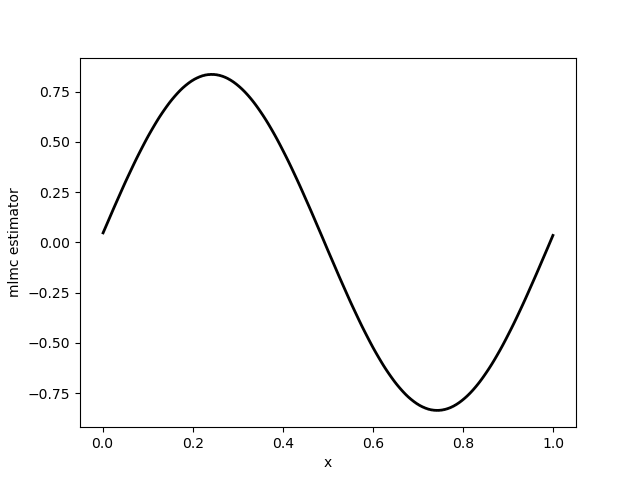
\includegraphics[width=75mm]{mlmc_mean_interp_uq}
  \caption{\textit{Multilevel Monte Carlo estimator of the random system in Example 1.}}
\end{figure}
\begin{figure}
  \centering
  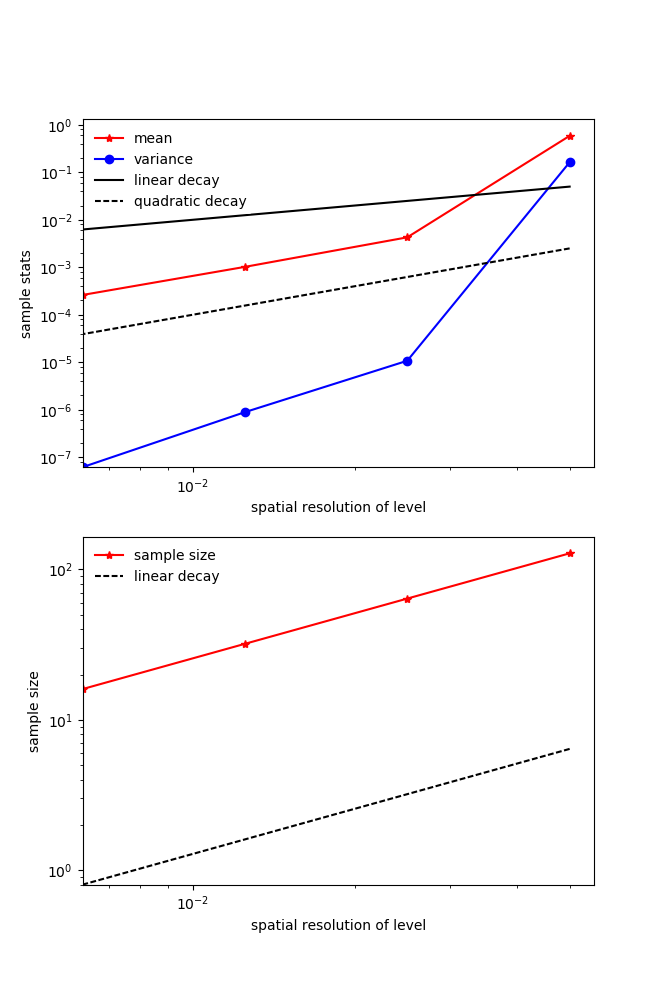
\includegraphics[width=75mm]{sample_stats_interp_uq}
  \caption{\textit{Sample statistics and sample sizes of each level in the multilevel Monte Carlo estimator of the random system in Example 1.}}
\end{figure}


\bibliography{refs}

\end{document}

\endinput


%%% Local Variables: 
%%% mode: latex
%%% TeX-master: t
%%% TeX-source-specials-mode: t
%%% TeX-PDF-mode: t
%%% End: 
